\documentclass[../report/report.tex]{subfiles}
%\usepackage{algpseudocode}
\begin{document}

\subsection{Usupervised learning}
The results of experiments on toy models suggest that the initial unsatisfactory results with naive mean field approaches \cite{tieleman2008training} might be greatly improved if add additional terms responsible for better estimation of (connections) between the spins.

\cite{dayan1999unsupervised}

Our general goal is to maximize the probability of $\mathcal{D}$ under the MRF distributions -- thus we are looking for the vector of parameters $\mathbf{\theta}$ that maximize the likelihood given the training data, i.e.
\begin{align}
\begin{split}
\max_{\mathbf{\theta}} \ln \mathcal{L}(\mathbf{\theta}| \mathcal{D}) = \max_{\mathbf{\theta}}  \ln \prod_{i=1}^N p(\mathbf{v}_i |\mathbf{\theta}) = \max_{\mathbf{\theta}} \sum_{i=1}^N \ln p(\mathbf{v}_i |\mathbf{\theta} )
\end{split}
\end{align}
In most of the cases, it is not possible to find the analytical solution for the maximum likelihood parameters and we need to resort to some approximation methods.



\subsection{Unsupervised Pre-training of Neural Networks}
add Erham here
\subsection{Training of Boltzmann Machines}
As it 

\begin{align}
\begin{split}
\mathbf{\theta}^{t+1} = \mathbf{\theta}^{t} + \eta  \frac{\partial}{\partial \mathbf{\theta}^t}  \ln \mathcal{L}(\mathbf{\theta}| \mathcal{D}) 
\end{split}
\end{align}
This relies on the fact that the gradient w.r.t. parameters $\mathbf{\theta}$ informs us how fast function increases in the current point $\mathbf{\theta}^{t}$. By taking appropriately small learning rate, these iterative updates might converge to the maximum of the function. However, there is no guarantees that this procedure will lead to obtaining global maximum.

TODO - stochastic gradient descent - theoretical results - writeabout it and read theoeretical results.

Learning Restricted Boltzmann machines relies on  gradient ascent of the log-likelihood. The gradient of the log-likelihood from given a training example $\mathbf{v}$ takes the form:
\begin{align}
\begin{split}
\frac{\partial \log \mathcal{L}(\mathbf{\theta  | \mathbf{v}})}{\partial \mathbf{\theta}} & = \frac{\partial \mathcal{F}^c }{\partial \mathbf{\theta}} - \frac{\partial \mathcal{F} }{\partial \mathbf{\theta}} \\
& = - \frac{\sum_{\mathbf{h}} e^{-E(\mathbf{v,h})} \frac{\partial E(\mathbf{v,h})}{\partial \mathbf{\theta}}}{\sum_{\mathbf{h}} e^{-E(\mathbf{v,h})}} + \frac{\sum_{\mathbf{v, h}} e^{-E(\mathbf{v,h})} \frac{\partial E(\mathbf{v,h})}{\partial \mathbf{\theta}}}{\sum_{\mathbf{v, h}} e^{-E(\mathbf{v,h})}} \\
& = - \sum_\mathbf{h} p(\mathbf{h} | \mathbf{v}) \frac{\partial E(\mathbf{v,h})}{\partial \mathbf{\theta}} +  \sum_\mathbf{v, h} p(\mathbf{v}, \mathbf{h}) \frac{\partial E(\mathbf{v,h})}{\partial \mathbf{\theta}} \\
& =  - \mathbb{E}_{p(\mathbf{h} | \mathbf{v})} \left( \frac{\partial E(\mathbf{v,h})}{\partial \mathbf{\theta}} \right) + \mathbb{E}_{ p(\mathbf{v,h}) } \left( \frac{\partial E(\mathbf{v,h})}{\partial \mathbf{\theta}} \right)
\end{split}
\end{align}

As we can see the gradient is the difference of two expectations -- the expected value of the gradient of the energy function under the model distribution and under the conditional distribution of the hidden variables given the observed variables $\mathbf{v}$. Thanks to the restriction imposed on the structure of the BM, the first term can be computed analytically \ref{eq:freeEnergy}. However, as it was mentioned previously, direct calculations of the second term leads to the complexity that is exponential in the number of variables in the model.

\subsection{MCMC Sampling}
The 
    
 \subsection{Contrastive Divergence}
 \subsubsection{Persistent CD}   
   \subsection{Learning in the TAP case}
    \subsubsection{Gradients}

Eq. 11. Gradients:

$$w_{ij}^{t+1} = w_{ij}^{t} + \eta \triangle w_{ij}^{t+1}$$

$$ \triangle w_{ij}^{t+1} \propto \frac{\partial \mathcal{L}}{\partial w_{ij}} \simeq -\frac{\partial F}{\partial w_{ij}} - \frac{\partial F^{EMF}}{\partial w_{ij}}$$

\begin{align*}
\begin{split}
\frac{\partial F^{EMF}}{\partial w_{ij}} = & -m_i^v m_j^h - w_{ij}^t(m_i^v - (m_i^v)^2)(m_j^h - (m_j^h)^2) \\
 & - 2w_{ij}^2 (m_i^v - (m_i^v)^2)(\frac{1}{2} - m_i^v)(m_j^h - (m_j^h)^2)(\frac{1}{2} - m_j^h)
\end{split}
\end{align*}

$$\frac{\partial \mathcal{L}}{\partial a_i} = \frac{\partial F^{EMF}}{\partial a_i} = -m_i^v$$

$$\frac{\partial \mathcal{L}}{\partial b_j} = \frac{\partial F^{EMF}}{\partial b_j} = -m_j^h$$

 
An example of such structure presents Figure \ref{fig:BM}.
\subsection{Approximating the likelihood}
TODO - describe problems and procedure.

\subsubsection{Pseudo approximation}
The problems mentioned above makes training such structure very difficult because we cannot observe directly progress along learning. Thus, we need to resort to some approximations. One of the most popular approaches is due to Besag \cite{besag1972nearest}.
Consider the following approximation:
\begin{equation}
P(\mathbf{s}) = \prod_i p(s_i| s_1,...,s_{i-1}) \approx \prod_i p(s_i | s_1, ..., s_{i-1}, s_{i+1},..., s_n) = \prod_i p(s_i| s_{-i})
\end{equation}
where the first equation comes from the chain rule. Here we assume that particular marginals given all other dimensions are independent of each other.
\begin{theorem}
TODO: Assume that $\mathbf{x}$ is generated I.ID. by a distribution $p(\mathbf{x};\mathbf{\theta})$.
\end{theorem}
	
If the analysed phenomena has many dimensions this approximation is still computationally expensive. Thus, another step is to choose only one marginal as a proxy, i.e.
\begin{equation}
\log PL(\mathbf{s}) = N \mathbb{E}\left(\log P(s_i | \mathbf{s}_{-i}) \right),
\end{equation}
where $i \sim U(1, N)$.

In the case of the analysed model we obtain the following form using Monte Carlo approximation (TODO: monte carlo approximation):
\begin{equation}
\log PL(\mathbf{s}) \approx N \log \left( \frac{\exp\{- F(\mathbf{s})\}}{\exp\{-F(\mathbf{\hat{s}})\} + \exp\{- F(\mathbf{s})\}} \right),
\end{equation}
where $\mathbf{\hat{s}}$ represents the vector $\mathbf{s}$ with $i$-th variable of flipped, i.e. $1-s_i$.

\subsection{Real scale model}
\subsubsection{MNIST data set}
\subsection{Comparison}


In order to test the efficiency of the EMF learning algorithm I used three approximations of $\ref{eq:varFreeEnergy}$ -- at first-order (MF), second-order (TAP2) and third order (TAP3). 

%lap

All trained models used the same set-up of free parameters. The purpose of this experiment is to compare different RBM trainings thus following \cite{gabrie2015training} I didn't use the adaptive learning rate which was set to $0.005$, learning was performed using mini-batch learning with $100$ training points per batch. The couplings matrix was randomly initialised using normal distribution with zero mean and variance set to $0.01$. This allows to compare the procedures in the their "raw" forms. 

However, the EMF approximation was performed around the infinite temperature were the spins are independent. This means that the couplings should have small values -- this can be enforced using regularization which at the same times allows for a better regularization. From probabilistic perspective it can be seen as adding a weighted prior over the parameters (maximum a posteriori). This leads to a new criterion which will be maximized of the form:
\begin{align}
\begin{split}
E(\theta, \mathcal{D}) = \ln \mathcal{L}(\mathbf{\theta}| \mathcal{D}) - \lambda R(\theta).
\end{split}
\end{align}
In all experiments I used Laplacian prior $R(\theta) = \| \theta \|_1$ ($L1$ regularization) with the weight $\lambda$ set to $0.01$. 

Figure \ref{fig:validLL} presents
\begin{figure}[!htb]
 %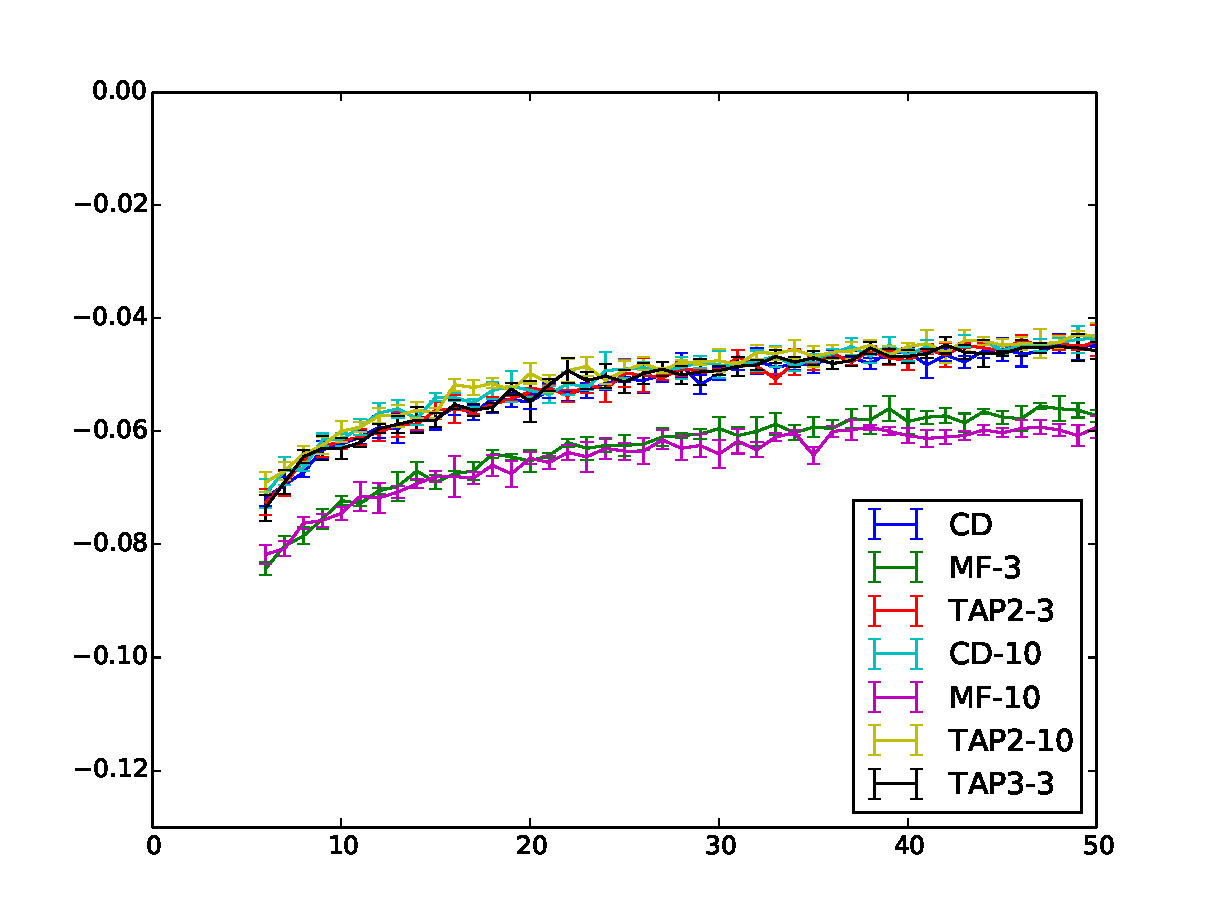
\includegraphics[width=\linewidth]{../../../Code/DRBM/scripts/validLL}
 \label{fig:validLL}
  \caption[1]{Pseudo LL.}
\end{figure}
COmment
Figure \ref{fig:validEMF} shows
\begin{figure}[!htb]
% 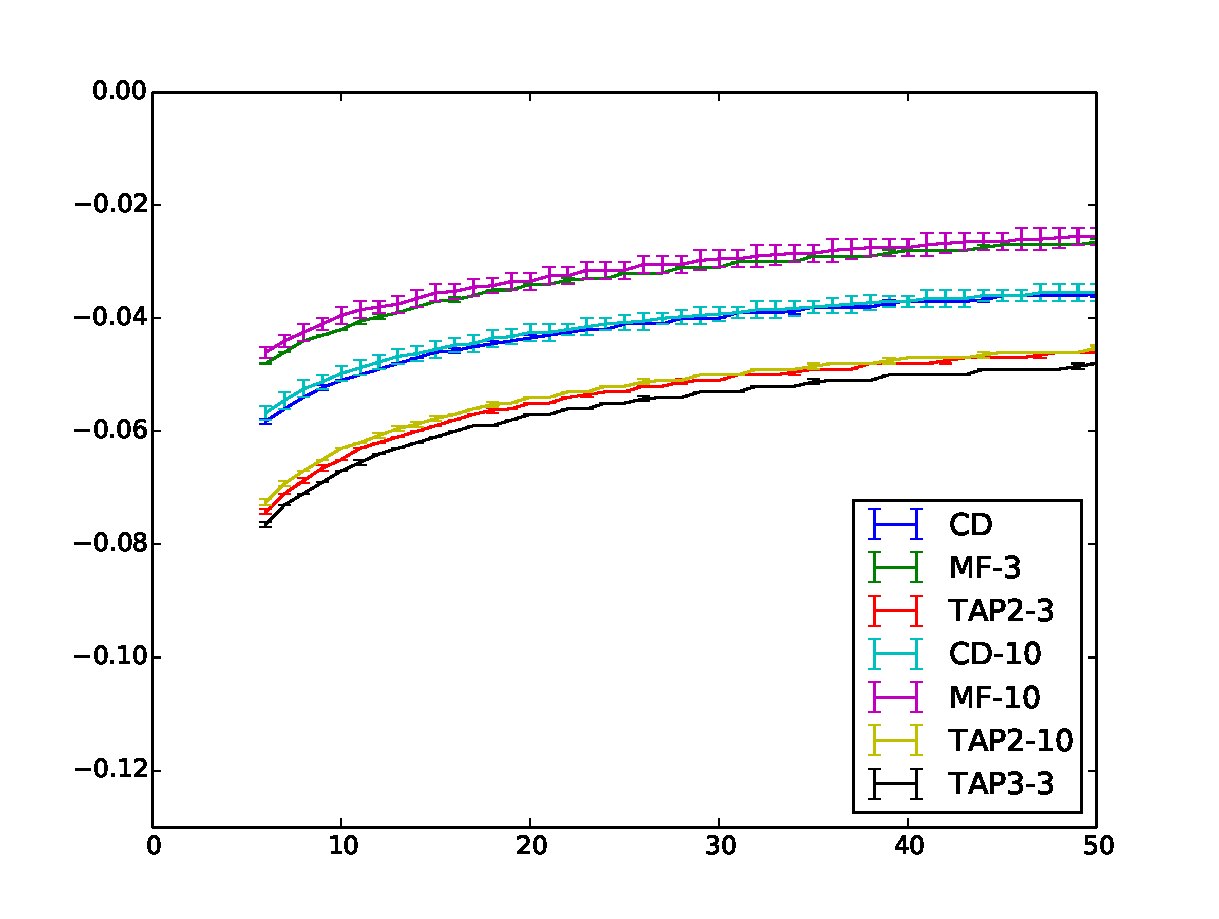
\includegraphics[width=\linewidth]{../../../Code/DRBM/scripts/validEMF}
  \caption[1]{EMF LL.}
\end{figure}
comment
\end{document}
